Este capítulo descreve a metodologia adotada para investigar a formação e impacto de câmaras de eco na rede de usuários da aplicação Colab. A pesquisa é estruturada de forma iterativa e incremental, permitindo que cada etapa informe e refine as subsequentes.

\section{Natureza da Pesquisa}

A pesquisa adota uma abordagem tanto descritiva quanto exploratória, conforme delineado por \cite{2008_Yin_BOOK} e \cite{2007_Babbie_BOOK}.

A pesquisa descritiva, como sugerido por \cite{2007_Babbie_BOOK}, é empregada quando o objetivo é descrever características de um fenômeno ou a relação entre variáveis. No contexto deste estudo, a abordagem descritiva é utilizada para categorizar e detalhar os usuários do Colab, fornecendo uma representação clara e sistemática dos mesmos. Esta metodologia é particularmente útil para estabelecer um panorama claro do comportamento dos usuários, suas interações e padrões de linguagem, formando assim a base para análises subsequentes.

Por outro lado, a pesquisa exploratória, conforme descrito por \cite{2008_Yin_BOOK}, é frequentemente empregada quando o pesquisador tem pouco ou nenhum conhecimento prévio sobre o fenômeno em estudo. Ela busca descobrir padrões, ideias ou hipóteses, em vez de testar uma hipótese predefinida. No caso desta pesquisa, a abordagem exploratória é crucial para identificar e compreender as câmaras de eco dentro da rede do Colab, um fenômeno ainda pouco explorado na literatura. Esta abordagem permite uma investigação flexível, adaptando-se à medida que novas descobertas emergem.

A combinação dessas duas abordagens é estratégica. Enquanto a pesquisa descritiva fornece uma base sólida e detalhada sobre os usuários e suas interações, a pesquisa exploratória permite a descoberta de novos insights e compreensões sobre as câmaras de eco. Esta combinação maximiza a profundidade e amplitude da análise, garantindo que tanto os aspectos bem definidos quanto os emergentes do fenômeno sejam adequadamente abordados.

\section{Universo e Amostra}
Os dados utilizados são oriundos do aplicativo Colab, representando um universo de [X usuários] no período de [data de início] a [data de fim] cobrindo as cidades de Caruaru, Rio de Janeiro, Recife, Niterói, Mesquita e Santo André. Nessa amostragem os usuários realizaram [X postagens] e [X comentários] num total de [X interações] analisadas.

\section{Coleta de Dados}
Os dados foram fornecidos pelo aplicativo Colab em formato CSV. Estes incluem listas de arestas, que representam as conexões entre os usuários, informações sobre o comportamento dos usuários, suas interações e postagens, além de dados demográficos e geográficos. Os dados foram anonimizados e não contêm informações pessoais dos usuários. O modelo dos dados e os preprocessamentos realizados são detalhados no \autoref{sec:modelo_de_dados}.

\section{Procedimentos de Análise}
\begin{itemize}
	\item \textbf{Análise de Redes Sociais:} Utilizando técnicas de ciência de dados e análise de grafos para identificar estruturas e características da rede Colab.
	\item \textbf{Classificação de Usuários:} Serão empregadas técnicas de processamento de linguagem natural e aprendizado de máquina supervisionado para classificar postagens e comportamentos dos usuários.
	\item \textbf{Detecção de Câmaras de Eco:} Adaptação das heurísticas propostas por \cite{2023_Atiqi_BOOK} ao contexto do Colab, combinadas com técnicas de análise de redes e teoria dos grafos.
	\item \textbf{Simulações:} A Modelagem Baseada em Agentes (ABM) e simulações de Monte Carlo serão usadas para avaliar o impacto de diferentes cenários e intervenções na formação de câmaras de eco.
\end{itemize}

\begin{figure}
	\centering
	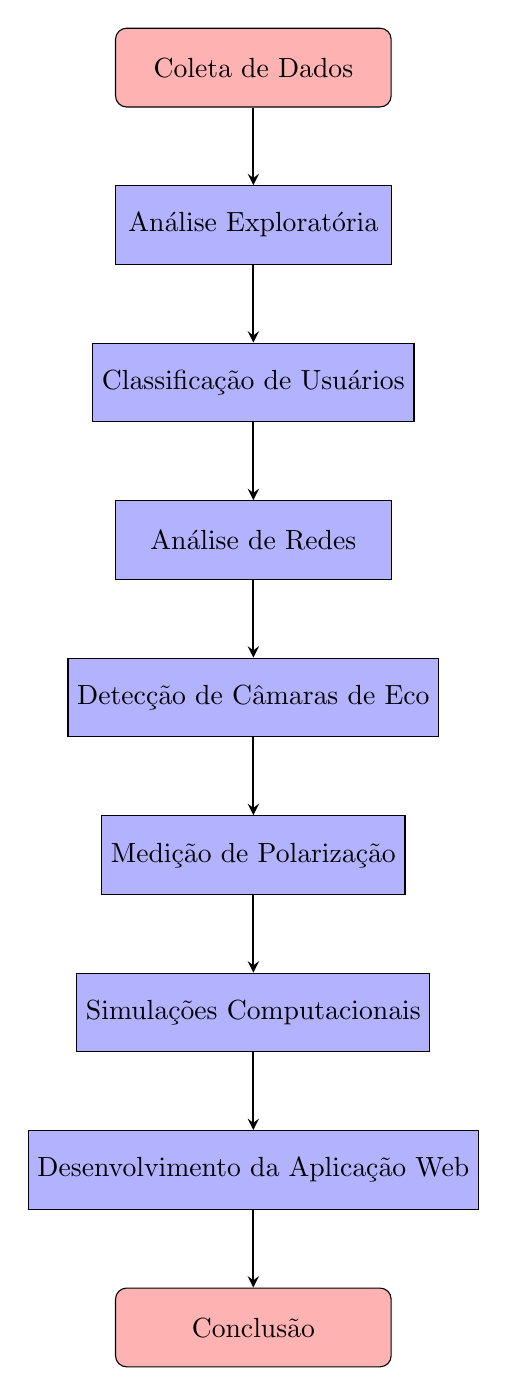
\begin{tikzpicture}[node distance=2cm]
		% Estilos para os nós
		\tikzstyle{startstop} = [rectangle, rounded corners, minimum width=3.5cm, minimum height=1cm, text centered, draw=black, fill=red!30]
		\tikzstyle{process} = [rectangle, minimum width=3.5cm, minimum height=1cm, text centered, draw=black, fill=blue!30]
		\tikzstyle{arrow} = [thick,->,>=stealth]
		% Nós
		\node (start) [startstop] {Coleta de Dados};
		\node (proc1) [process, below of=start] {Análise Exploratória};
		\node (proc2) [process, below of=proc1] {Classificação de Usuários};
		\node (proc3) [process, below of=proc2] {Análise de Redes};
		\node (proc4) [process, below of=proc3] {Detecção de Câmaras de Eco};
		\node (proc5) [process, below of=proc4] {Medição de Polarização};
		\node (proc6) [process, below of=proc5] {Simulações Computacionais};
		\node (proc7) [process, below of=proc6] {Desenvolvimento da Aplicação Web};
		\node (stop) [startstop, below of=proc7] {Conclusão};
		% Setas
		\draw [arrow] (start) -- (proc1);
		\draw [arrow] (proc1) -- (proc2);
		\draw [arrow] (proc2) -- (proc3);
		\draw [arrow] (proc3) -- (proc4);
		\draw [arrow] (proc4) -- (proc5);
		\draw [arrow] (proc5) -- (proc6);
		\draw [arrow] (proc6) -- (proc7);
		\draw [arrow] (proc7) -- (stop);
	\end{tikzpicture}
	\caption{Diagrama ilustrando os passos da metodologia.}
\end{figure}

\section{Ferramentas e Softwares}
Serão utilizados softwares específicos para análise de redes sociais, como Gephi ou NodeXL, e linguagens de programação, como Python ou R, para análises mais detalhadas. Bibliotecas de aprendizado de máquina, como Scikit-learn, TensorFlow ou PyTorch, serão empregadas para treinamento de modelos.

\section{Aspectos Éticos}
A pesquisa garante a anonimidade das informações pessoais dos usuários. Todos os dados sensíveis serão tratados com precaução, assegurando a integridade e privacidade dos participantes.

\section{Limitações}
Os resultados e conclusões desta pesquisa são específicos do universo do Colab, o que pode limitar sua generalização para outras plataformas ou contextos.